\documentclass{llncs}
\pagestyle{plain}
%\usepackage[margin=2.5cm]{geometry}
\usepackage[pdftex]{graphicx}
\usepackage{caption}
\usepackage{subcaption}
\usepackage[rightcaption]{sidecap}
\usepackage{float}
\usepackage[ruled, vlined, linesnumbered]{algorithm2e}
\SetAlgoSkip{bigskip}
\usepackage{hyperref}
\usepackage{amsmath}
\usepackage{titling}
\usepackage{soul}
\usepackage{cite}

\usepackage{fancyhdr}
\pagestyle{fancy}
\fancyhf{}
\lhead{Swarm Intelligence}
\rhead{Winter 2014/15}
\cfoot{\thepage}

\setlength{\droptitle}{-4em}
\title{Collective Decision Making with Heterogeneous Agents}
\author{Syam Ajay Simha Gullipalli\\
		Universit\"at Paderborn\\
		\texttt{syam@mail.uni-paderborn.de}}
\date{\today}

\begin{document}
	\maketitle
	\thispagestyle{fancy}
	
	\section{Introduction}
	Choosing an option from a choice of $N$ alternatives based on quality metrics is easy if every alternative is processed. The agents used to evaluate the quality metrics should have immense processing capabilities, because the time and computational power it takes to choose the best increases with the number of alternatives which is known as \textit{best-of-n} decision problem. Multiple distributed agents with simple capabilites may dominate a single central agent with enormous capabilities. Natural computing, an emerging technology which takes inspiration from nature, has its own advantages in solving complex problems. This paper focuses on swarm robotics, a part of natural computing which uses relatively simple, distributed and self-organized robots (agents) to accomplish complex tasks. The biggest advantage of distributed agents over a central agent is, the distributed agents are not prone to single point of failure.
	
	This paper presents a solution to tackle a problem when the agents are heterogeneous. There are four rooms $r_i$ where $i \in [0,3]$ connected to the edges of a central room. The agents can differentiate the room by finding a color at the entrance of the romm. The central room has an entrance to each room. Each room has its quality metrics; ground color ($v_G$), light intrensity ($v_L$), and objects ($v_O$). The task is to choose the room with high average value of these three metrics. The heterogeneous robots used here are of two types; Robots with ground sensor to evaluate ground color (type G), and robots with light sensor to evaluate the light intensity (type L). Robots of both type G and L have omnidirectional camera to detect objects around it. Each metric is a value between 0 and 1. Each room can have a minimum of 2 and maximum of 12 objects. The objects evaluation metric ($v_O$) using the number of objects ($n_O$) is calculated using equation \eqref{eq:vOEval} to have a value between 0 and 1.
	
	%EQUATION: v_O evaluation
	\begin{equation}
		\centering
		v_O = 0.1(n_O) - 0.2
		\label{eq:vOEval}
	\end{equation}
	
	\section{Solution from Honeybee Swarms} \label{sec:introduction}
	Exchanging information among the agents in a swarm during collective decision making is an important task. An agent assess the quality of information upon new information to take individual decision. The decisions of individual agents emerges to a global behavior of every agent to agree on the same decision. Since, the communication capabilities of swarm robots are limited, it is impossible to exchange the complete knowledge of every single metric among all robots. The decision making is difficult when the robots are heterogeneous, because each agent can percieve a limited knowledge. Due to limited communication and no complete knowledge, the robots have to depend on simple information like opinion.
	
	The solution implemented follows the ideas of "The Weighted Voter Model" presented in literature \cite{Valentini:2014:SCD:2615731.2615742}. It is a hybrid method of combining house hunting behavior of honeybees and opinion dynamics. During house hunting, honeybees individually \textit{survey} and collect information about the available \textit{sites}. When a honeybee chooses a site, it comes back to the \textit{nest} and tries to influence the neighbors to survey the site by \textit{waggle dances}. The waggle dance encodes the information about available metrics like distance, direction, quality etc. This house hunting behavior is applied on classic voter model in which a random opinion is adopted by a random agent in each step. When waggle dance ends, the honeybee adopts an \textit{opinion} of random neighbor and surveys the site. This procedure eventually makes all the honeybees to have the same opinion of site. The positive feedback here is the duration of the waggle dance which is directly proportional to the quality of the opinion. Therefore, if the qulatiy of site is high, the agent invests larger time on waggle dance to influence more number of agents to have the same opinion.

	\section{State Machine}	\label{sec:stateMachine}
	For the convenience of comparing the configuraion of current task to honeybees behavior, the central room is considered as nest and the rooms connected to it's edges are considered as sites. The transitions of different states for the solution construction is shown in figure \ref{fig:stateMachine}. Initially, robot has no opinion, so it is set to INIT to have an opinion. AVOID state is used to avoid collisions. SURVEY state sets the behavior of robot to go to the site of opinion and evaluate metrics perceived. WAGGLE state sets the behavior of robot to get into the nest and broadcast it's opinion. All possible transitions of these states are:
	
	%FIGURE: State Machine
	\begin{figure}[h!]
		\centering
		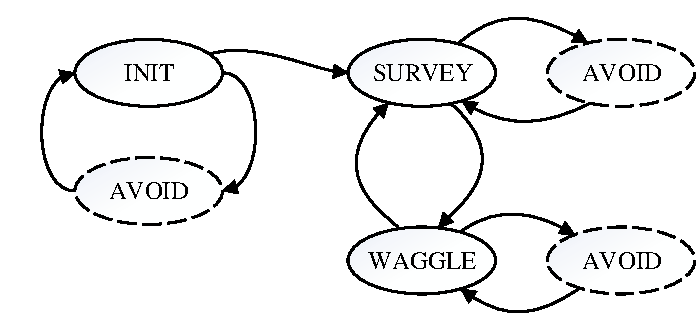
\includegraphics[width=0.7\textwidth]{IMG/StateMachine}
		\caption{State machine for collective decision making using house hunting behavior of honeybees.}
		\label{fig:stateMachine}
	\end{figure}
	
	\subsection{Any state to AVOID}
	Collision avoidance mechanism is a high priority task to avoid physical damages to robots. The robot transforms to AVOID state from any state when a collision is detected.
	
	\subsection{AVOID to previous state}
	When a collision is avoided, the robot transforms to the previous state to perform desired task. The robot has to preserve the current state before transforming to AVOID to resume the state again after collision avoidance.
	
	\subsection{INIT to SURVEY}
	Initially, a robot has no opinion which is initialized to INIT state. Upon having an opinion, the robot transforms to SURVEY state to percieve the metrics of the opinion. This transition is performed only once during exection.
	
	\subsection{SURVEY to WAGGLE}
	Upon time out of the SURVEY state, robot transforms to WAGGLE state to broadcast opinion and influence it's neighbors.
	
	\subsection{WAGGLE to SURVEY}
	Upon time out of the WAGGLE state, robot adopts opinion from a random neighbor and enters SURVEY state to perceive the quality of site. When ever a robot transforms from WAGGLE to SURVEY state, it considers the problem as \textit{binary decision problem} instead of \textit{best-of-n} decision problem, because it can choose only between two opinions, the opinion it has already and the opinion of a (random) single nighbor.
	
	
	\section{Implementation}
	The behavior of the robot is changed by set and reset of the basic flags \texttt{is\_room\_sensed}, \texttt{is\_at\_entrance}, and \texttt{is\_entered\_room} flags as in flowchart shown in figure \ref{fig:flowChart}. This flowchart can be easily transformed into a basic structure of algorithm depicted in \ref{alg:pseudocode}. The flags are set and reset within the function definitions to change the behavior of robots. For simplicity, the collision avoidance mechanism is considered as an internal mechanism of robots, therefore not shown in the flowchart or algorithm, although it is designed as a separate state.
	
	%FIGURE: Flow Chart
	\begin{figure}[h!]
		\centering
		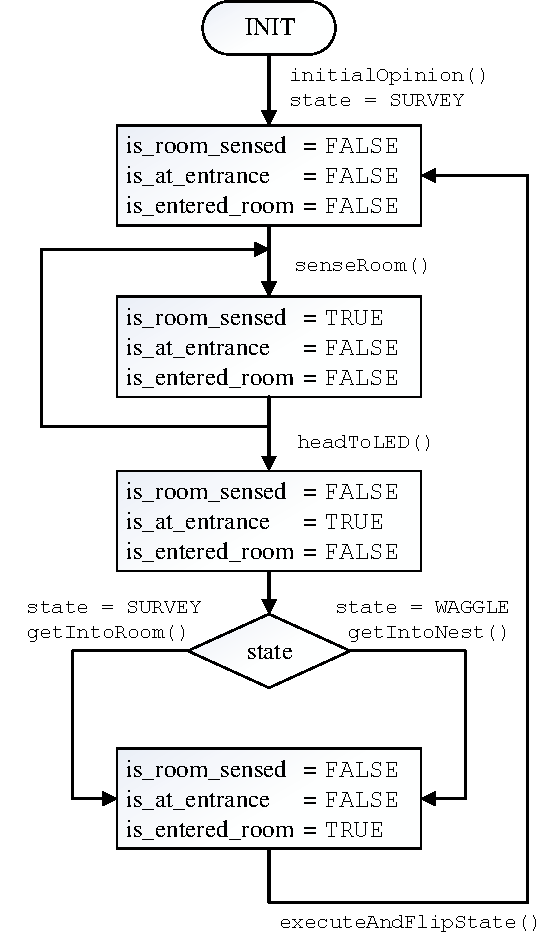
\includegraphics[width=0.7\textwidth]{IMG/FlowChart}
		\caption{Flowchart showing transitions of important flags to change state and behavior of a robot.}
		\label{fig:flowChart}
	\end{figure}
	
	%ALGORITHM: Pseucode
	\begin{algorithm}[h!]
		state = INIT\tcc*[r]{Initial state}
		initialOpinion()\tcc*[r]{Have an initial opinion}
		state = SURVEY\tcc*[r]{Change to SURVEY state when robot has an opinion}
		\uIf(\tcc*[h]{Recognized the room of opinion}){is\_room\_sensed}{
			headToLED()\tcc*[r]{Go towards the room sensed}
		}
		\uElseIf(\tcc*[h]{Close to the room of opinion}){is\_at\_entrance}{
			\uIf(\tcc*[h]{SURVEY state}){state == SURVEY}{
				getIntoRoom()\tcc*[r]{Enter into the room}
			}
			\Else(\tcc*[h]{WAGGLE state}){
				getIntoNest()\tcc*[r]{Exit the room to enter the nest}
			}
		}
		\uElseIf(\tcc*[h]{In the desired room}){is\_entered\_room}{
			executeAndFlipState()\tcc*[r]{Perform activities of current state and flip the state on timeout}
		}
		\Else(\tcc*[h]{Room not sensed}){
			senseRoom()\tcc*[r]{Search for the room matching the opinion}
		}
	\caption{Transformed pseudocode from the flochart in image \ref{fig:flowChart}.}\label{alg:pseudocode}
	\end{algorithm}
	
	
	The basic functions of the robt are:
	\subsection*{\texttt{detectCollision()}}
	Detect collisions ahead. If a collision is detected, preserve the current state before changing to AVOID state.
	
	\subsection*{\texttt{avoidCollision()}}
	Avoid collision if a collision is detected by \texttt{detectCollision()}. Resume the previous state when collision is avoided.
	
	\subsection*{\texttt{initialOpinion()}}
	Get an initial opinion of which site to survey. For the experiment results presented, each room has assigned equal (or nearly equal if not possible) number of of robots. 
	\subsection*{\texttt{senseRoom()}}
	Find the site of the robot's opinion by detecting the LED color placed at the entrance of the site to change the heading. Set the flag \texttt{is\_room\_sensed} when detected the site to perform the next action.
	
	\subsection*{\texttt{headToLED()}}
	Go near the LED placed at the entrance of the site to make sure that the robot is moving into desired site or nest. When the robot is close enough to the desired LED, set \texttt{is\_at\_entrance}.
	
	\subsection*{\texttt{getIntoRoom()}}
	Get into the site (room) if the robot is close enough to the LED. This function is executed only when the robot is in SURVEY state. The robot finds the objects in the site and tries to go near the object to confirm that it has entered the site. Upon confirmation, set the flag \texttt{is\_entered\_room} to execute the actual behavior of SURVEY state.
	
	\subsection*{\texttt{getIntoNest()}}
	Get into the nest (central room) if the robot is close enough to the LED. This function is executed only when the robot is in WAGGLE state. The robot finds the LEDs placed at the entrance of the site other than the current opinion and tries to go away from the site towards those LEDs. When the robot is away a certain distance from the LED of current opinion, confirm that it has entered the nest. Upon confirmation, set the flag \texttt{is\_entered\_room} to execute the actual behavior of WAGGLE state.
	
	\subsection*{\texttt{executeAndFlipState()}}
	Set timer, the number of steps the robot has to execute the current state. If the current state is SURVEY, a uniform random integer value between 150 and 300 is taken as the number of steps the robot has to execute. If the current state is WAGGLE, an exponential value proportional to the average of metrics $v$ calculated using equation \eqref{eq:exTime} is set to the number of time steps $t$ the robot has to move before changing the state to SURVEY. The values of rate parameter $\lambda$ and weight $W$ are set to -2 and 40 respectiveley.
	
	\begin{equation}
		\centering
		t = W \lambda (1 - e^{-\lambda v})
		\label{eq:exTime}
	\end{equation}
	
	If the current state is SURVEY, assess the quality of the rooom by calling \texttt{updateMetrics()}. If current state is WAGGLE, broadcast it's opinion. On timeout, if the current state is WAGGLE then stop broadcasting the opinion and adopt an opinion from random neighbor. Flip the current state from SURVEY/WAGGLE to WAGGLE/SURVEY and reset all the flags \texttt{is\_room\_sensed}, \texttt{is\_at\_entrance}, \texttt{is\_entered\_room}.
	
	\subsection*{\texttt{updateMetrics()}}
	Update the metrics of the robot when best values found. The average of the metrics found $v$ is calculated as in equation \eqref{eq:avgMetric}.
	

	\begin{equation}
		\centering
		v = \left\{
		\begin{array}{l l}
		(v_G + v_O) / 2 & \quad \text{if type G robot}\\
		(v_L + v_O) / 2 & \quad \text{if type L robot}
		\end{array} \right.
		\label{eq:avgMetric}
	\end{equation}
	
	%Comparision
	\section{Analysis and Results}\label{sec:comparision}
	The results for 9 experiments by varying the robot count, each executed 5 sequential runs is presented in figures \ref{fig:plots123}, \ref{fig:plots456}, \ref{fig:plots789}. Every run in each experiment is executed for 5000 ticks. $T_G$ is the number of type G robots and $T_L$ is the number of type L robots. The left side bar graph on each plot shows the average of metrics of the original configuration on each room. The right side bar graph shows the opinions of the robots on each run.
	
	The results show that the robots try to choose room with high average of metrics irrespective of the average of only perceivable metrics (a robot may have a ground or light sensor value, but not both). Eventually, almost every robot agrees on the same room. If the difference between the average of metrics $v$ of each room is high, the robots perform better and may give optimal solution and also take less time for consensus. If these values are closer, the robots try to find near optimal solutions and may take larger time for consensus. Too many robots increases the time for the robots to agree on the same room, but initially they give many (near optimal) solutions, slowly decreasing the number of solutions by forming clusters. Too many robots is a good choice to find many better solutions rather than the single best solution.
	
	For the given configuration 20-25 robots of equal sizes of $T_G$ and $T_L$ is a good value to have a (near) optimal solution. The results vary by varying the ratio of $T_G$ and $T_L$. If the robot count of type G ($T_G$) is more compared to type L ($T_L$), the results favor the room with high ground sensor values.	
	
	
	%PLOTS: 1 2 3
	\begin{figure}[h!]
        \centering
        \begin{subfigure}[b]{0.25\textwidth}
                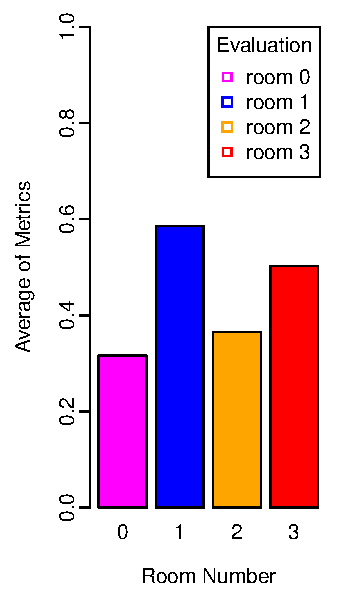
\includegraphics[width=\textwidth]{PLOT/EVAL/eval1}
                \caption{$T_G = 10$, $T_L = 10$}
                \label{fig:eval1}
        \end{subfigure}%
        \qquad
        \begin{subfigure}[b]{0.67\textwidth}
                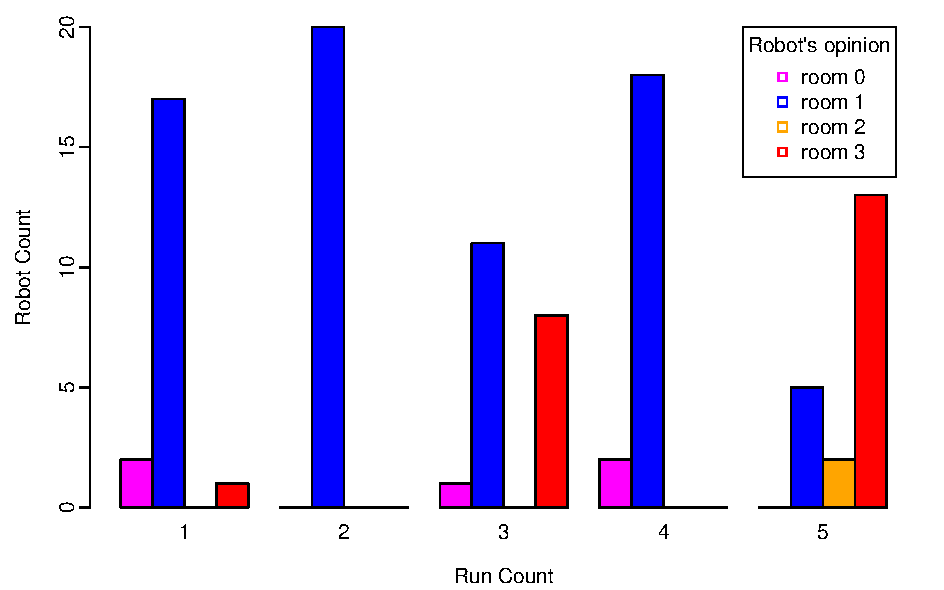
\includegraphics[width=\textwidth]{PLOT/EXP/exp1}
                \label{fig:exp1}
        \end{subfigure}
        
        \begin{subfigure}[b]{0.25\textwidth}
                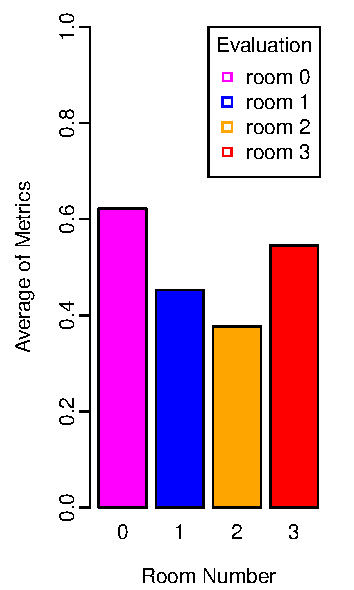
\includegraphics[width=\textwidth]{PLOT/EVAL/eval2}
                \caption{$T_G = 10$, $T_L = 10$}
                \label{fig:eval1}
        \end{subfigure}%
        \qquad
        \begin{subfigure}[b]{0.67\textwidth}
                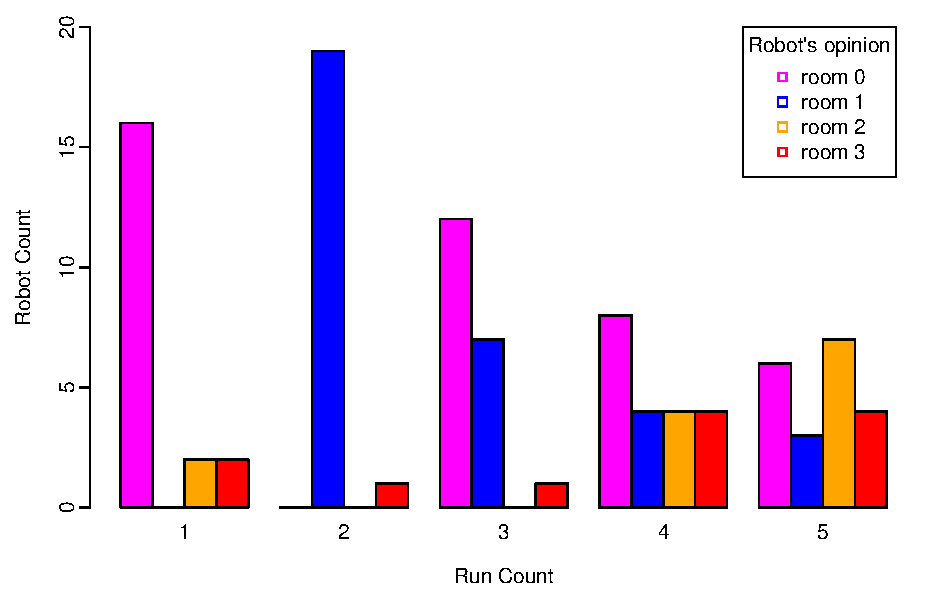
\includegraphics[width=\textwidth]{PLOT/EXP/exp2}
                \label{fig:exp1}
        \end{subfigure}
        
        \begin{subfigure}[b]{0.25\textwidth}
                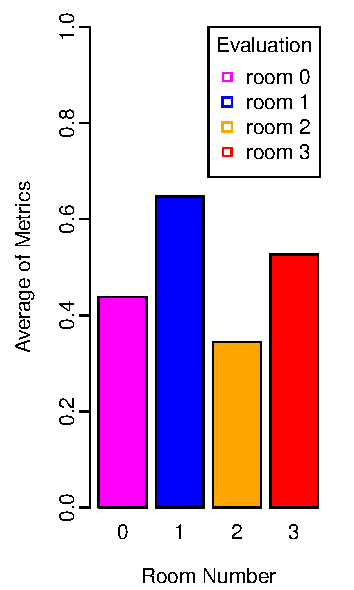
\includegraphics[width=\textwidth]{PLOT/EVAL/eval3}
                \caption{$T_G = 12$, $T_L = 13$}
                \label{fig:eval1}
        \end{subfigure}%
        \qquad
        \begin{subfigure}[b]{0.67\textwidth}
                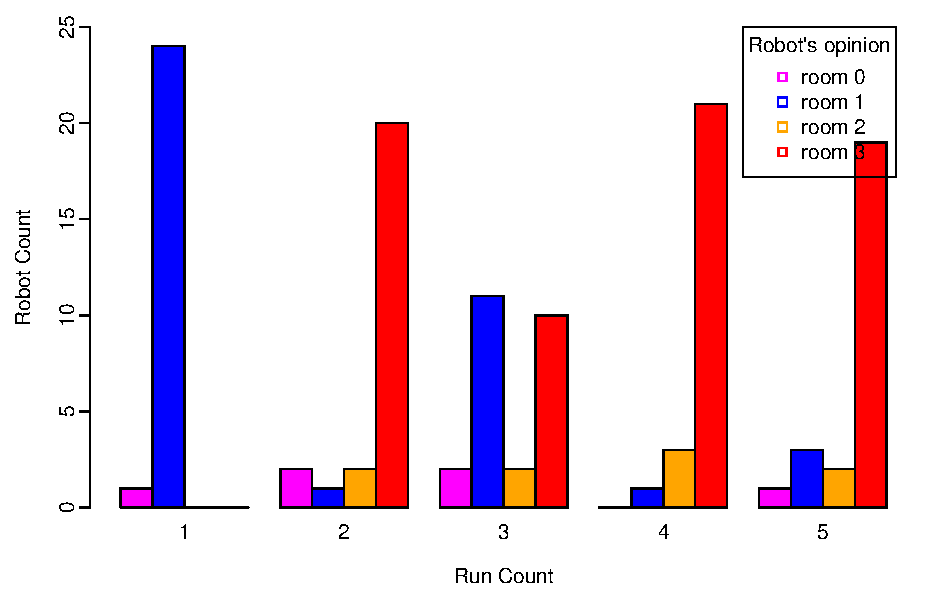
\includegraphics[width=\textwidth]{PLOT/EXP/exp3}
                \label{fig:exp1}
        \end{subfigure}
        
	\caption{Results of experiments on different configurations with (a) 20 robots, (b) 20 robots, and (c) 25 robots.}\label{fig:plots123}
	\end{figure}
	
	%PLOTS: 4 5 6
	\begin{figure}[h!]
        \centering
        \begin{subfigure}[b]{0.25\textwidth}
                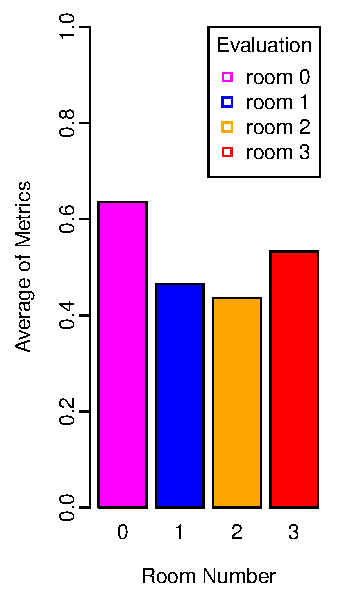
\includegraphics[width=\textwidth]{PLOT/EVAL/eval4}
                \caption{$T_G = 13$, $T_L = 12$}
                \label{fig:eval1}
        \end{subfigure}%
        \qquad
        \begin{subfigure}[b]{0.67\textwidth}
                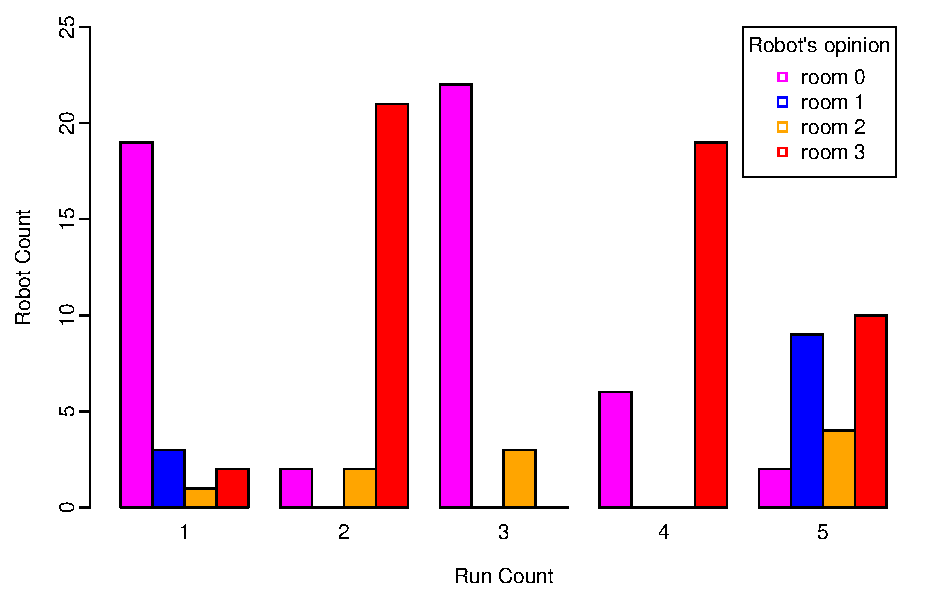
\includegraphics[width=\textwidth]{PLOT/EXP/exp4}
                \label{fig:exp1}
        \end{subfigure}
        
        \begin{subfigure}[b]{0.25\textwidth}
                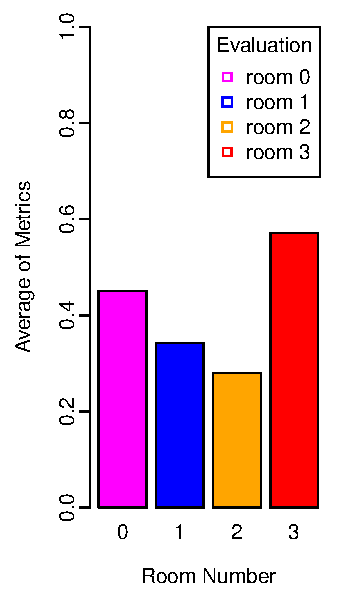
\includegraphics[width=\textwidth]{PLOT/EVAL/eval5}
                \caption{$T_G = 15$, $T_L = 15$}
                \label{fig:eval1}
        \end{subfigure}%
        \qquad
        \begin{subfigure}[b]{0.67\textwidth}
                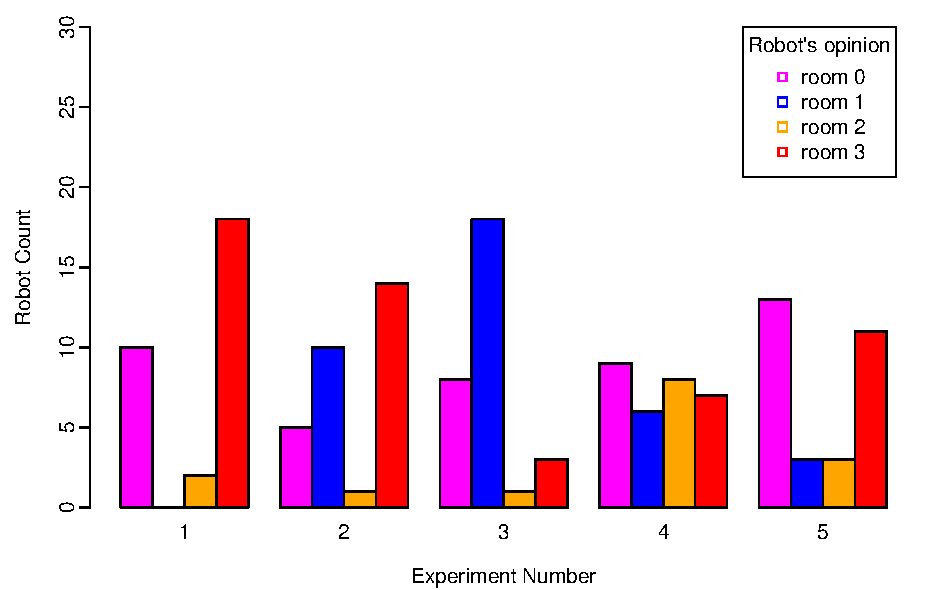
\includegraphics[width=\textwidth]{PLOT/EXP/exp5}
                \label{fig:exp1}
        \end{subfigure}
        
        \begin{subfigure}[b]{0.25\textwidth}
                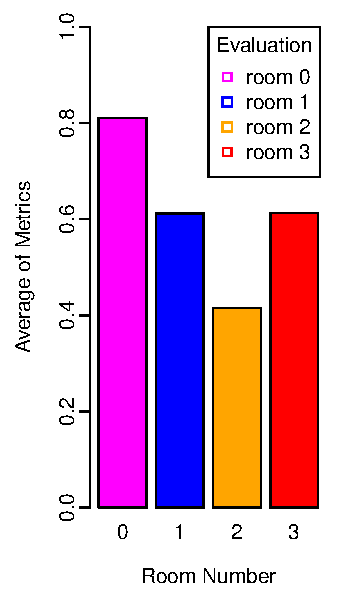
\includegraphics[width=\textwidth]{PLOT/EVAL/eval6}
                \caption{$T_G = 15$, $T_L = 15$}
                \label{fig:eval1}
        \end{subfigure}%
        \qquad
        \begin{subfigure}[b]{0.67\textwidth}
                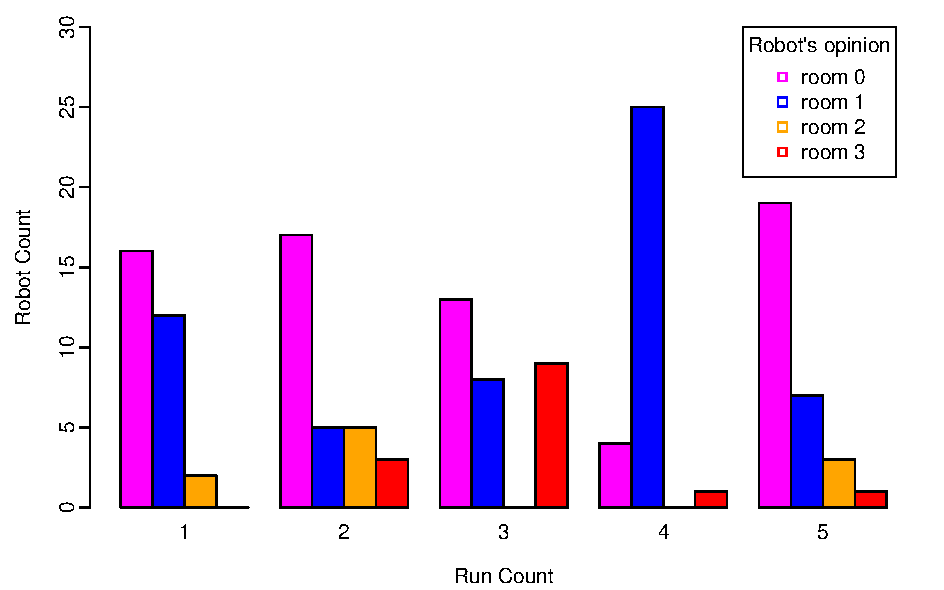
\includegraphics[width=\textwidth]{PLOT/EXP/exp6}
                \label{fig:exp1}
        \end{subfigure}
        
	\caption{Results of experiments on different configurations with (a) 25 robots, (b) 30 robots, and (c) 35 robots.}\label{fig:plots456}
	\end{figure}
	
		%PLOTS: 7 8 9
	\begin{figure}[h!]
        \centering
        \begin{subfigure}[b]{0.25\textwidth}
                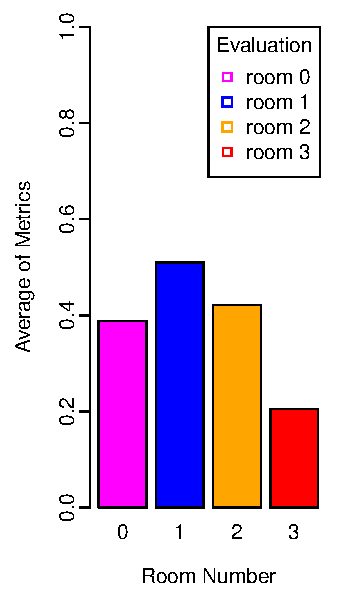
\includegraphics[width=\textwidth]{PLOT/EVAL/eval7}
                \caption{$T_G = 17$, $T_L = 18$}
                \label{fig:eval1}
        \end{subfigure}%
        \qquad
        \begin{subfigure}[b]{0.67\textwidth}
                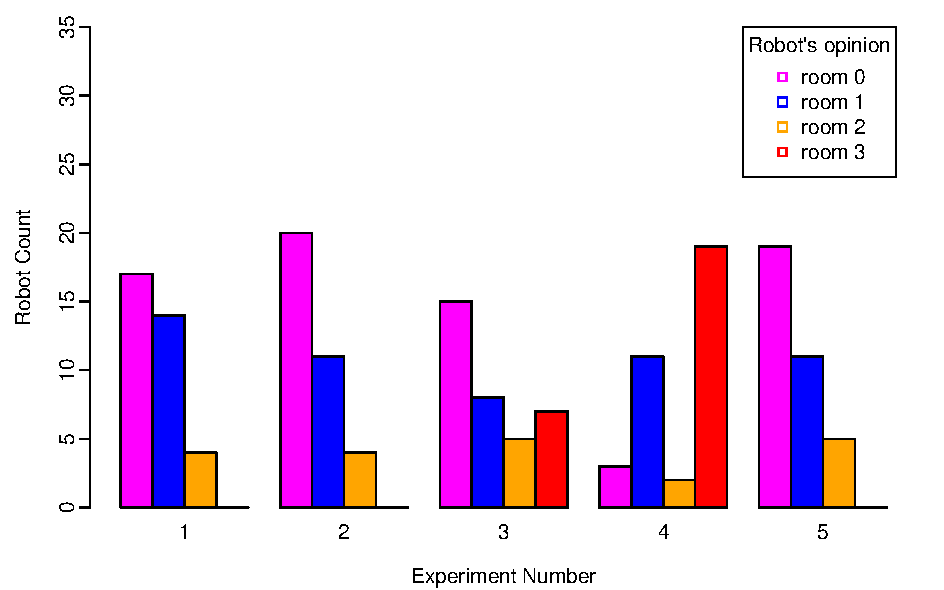
\includegraphics[width=\textwidth]{PLOT/EXP/exp7}
                \label{fig:exp1}
        \end{subfigure}
        
        \begin{subfigure}[b]{0.25\textwidth}
                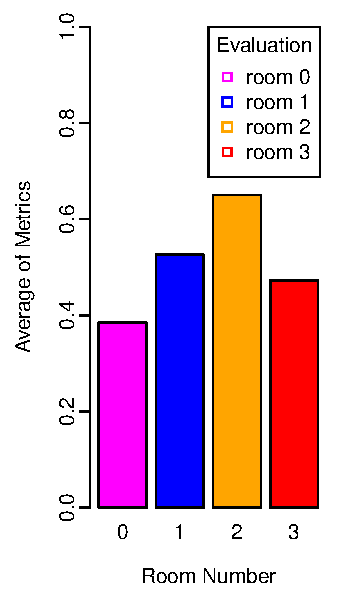
\includegraphics[width=\textwidth]{PLOT/EVAL/eval8}
                \caption{$T_G = 18$, $T_L = 17$}
                \label{fig:eval1}
        \end{subfigure}%
        \qquad
        \begin{subfigure}[b]{0.67\textwidth}
                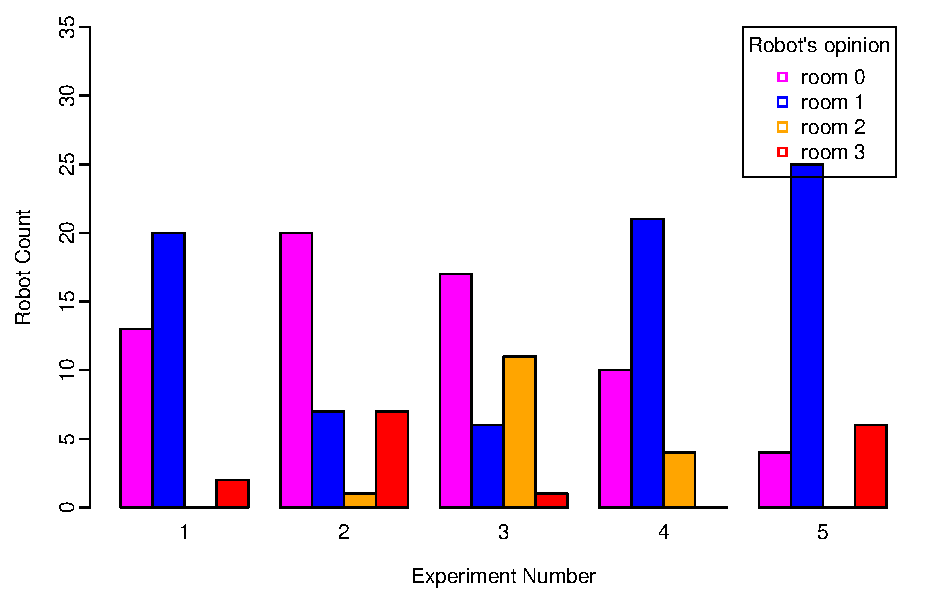
\includegraphics[width=\textwidth]{PLOT/EXP/exp8}
                \label{fig:exp1}
        \end{subfigure}
        
        \begin{subfigure}[b]{0.25\textwidth}
                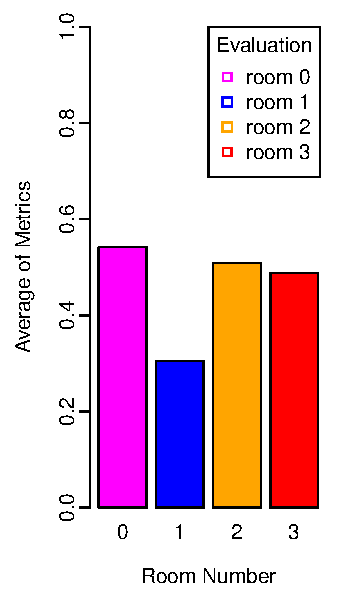
\includegraphics[width=\textwidth]{PLOT/EVAL/eval9}
                \caption{$T_G = 20$, $T_L = 20$}
                \label{fig:eval1}
        \end{subfigure}%
        \qquad
        \begin{subfigure}[b]{0.67\textwidth}
                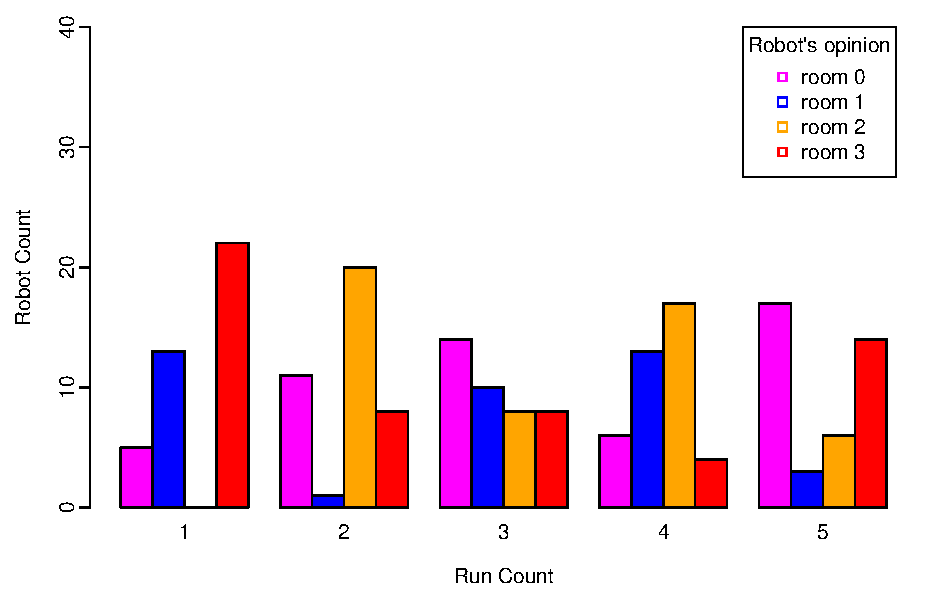
\includegraphics[width=\textwidth]{PLOT/EXP/exp9}
                \label{fig:exp1}
        \end{subfigure}
        
	\caption{Results of experiments on different configurations with (a) 35 robots, (b) 35 robots, and (c) 40 robots.}\label{fig:plots789}
	\end{figure}
	
	
	%Conclusion
	\section{Conclusion}\label{sec:conclusion}
	The hybrid method using house hunting behavior of honeybees and opinion dynamics for collective decision making suits well where the agents are heterogeneous, and have noisy sensors and limited communication capabilities. Since, the room entrance for each room in the given experiment configuration is a narrow passage, the random walk leads to congestion problem where robots spend a lot of time on collision avoidane if too many robots try to enter and exit the same room. Forming patterns to enter and exit the room for congestion conrtol instead of random walk may improve the quality and time complexity. The positive feedback mechanism here is, the amount of time a robot waggle dance is directly proportional to the quality of metrics. Exponential time for the waggle dance improves the quality of decision by spending much time on influencing other to choose better solution.
	
	
	\bibliographystyle{splncs}
	\bibliography{literature}
	\nocite{*}
	
\end{document}